\bta{研究平抛运动}

\begin{enumerate}
\renewcommand{\labelenumi}{\arabic{enumi}.}
% A(\Alph) a(\alph) I(\Roman) i(\roman) 1(\arabic)
%设定全局标号series=example	%引用全局变量resume=example
%[topsep=-0.3em,parsep=-0.3em,itemsep=-0.3em,partopsep=-0.3em]
%可使用leftmargin调整列表环境左边的空白长度 [leftmargin=0em]
\item
\exwhere{$ 2019 $ 年 $ 4 $ 月浙江物理选考}
采用如图所示的实验装置做“研究平抛运动”的实验。
\begin{figure}[h!]
\centering
\includesvg[width=0.23\linewidth]{picture/svg/GZ-3-tiyou-0443}
\end{figure}


\begin{enumerate}
\renewcommand{\labelenumi}{\arabic{enumi}.}
% A(\Alph) a(\alph) I(\Roman) i(\roman) 1(\arabic)
%设定全局标号series=example	%引用全局变量resume=example
%[topsep=-0.3em,parsep=-0.3em,itemsep=-0.3em,partopsep=-0.3em]
%可使用leftmargin调整列表环境左边的空白长度 [leftmargin=0em]
\item
实验时需要下列哪个器材 \tk{B} 
\threechoices
{弹簧秤}
{重锤线}
{打点计时器}


\item 
做实验时,让小球多次沿同一轨道运动,通过描点法画出小球平抛运动的轨迹。下列的一些
操作要求,正确的是 \tk{ACD} 
\fourchoices
{每次必须由同一位置静止释放小球}
{每次必须严格地等距离下降记录小球位置}
{小球运动时不应与木板上的白纸相接触}
{记录的点应适当多一些}

\item 
若用频闪摄影方法来验证小球在平抛过程中水平方向是匀速运动,记录下如图所示的频闪照
片。在测得 $ x_{1} $,$ x_{2} $,$ x_{3} $,$ x_{4} $ 后,需要验证的关系是 \tk{$x_{4}-x_{3}=x_{3}-x_{2}=x_{2}-x_{1}=x_{1}$} 。已知频闪周期为 $ T $,用下列
计算式求得的水平速度,误差较小的是 \tk{D} 
\begin{figure}[h!]
\centering
\includesvg[width=0.23\linewidth]{picture/svg/GZ-3-tiyou-0444}
\end{figure}

\fourchoices
{$\frac{x_{1}}{T}$}
{$\frac{x_{2}}{2 T}$}
{$\frac{x_{3}}{3 T}$}
{$\frac{x_{4}}{4 T}$}


\end{enumerate}



\newpage
\item 
\exwhere{$ 2019 $ 年物理北京卷}
用如图 $ 1 $ 所示装置研究平地运动。将白纸和复写纸对齐重叠并固定在竖直的
硬板上。钢球沿斜槽轨道 $ PQ $ 滑下后从 $ Q $ 点飞出,落在水平挡板 $ MN $ 上。由于挡板靠近硬板一侧较
低,钢球落在挡板上时,钢球侧面会在白纸上挤压出一个痕迹点。移动挡板,重新释放钢球,如此
重复,白纸上将留下一系列痕迹点。
\begin{figure}[h!]
\centering
\includesvg[width=0.23\linewidth]{picture/svg/GZ-3-tiyou-0445}
\end{figure}

\begin{enumerate}
\renewcommand{\labelenumi}{\arabic{enumi}.}
% A(\Alph) a(\alph) I(\Roman) i(\roman) 1(\arabic)
%设定全局标号series=example	%引用全局变量resume=example
%[topsep=-0.3em,parsep=-0.3em,itemsep=-0.3em,partopsep=-0.3em]
%可使用leftmargin调整列表环境左边的空白长度 [leftmargin=0em]
\item
下列实验条件必须满足的有 \tk{BD} 。

\fourchoices
{斜槽轨道光滑}
{斜槽轨道末段水平}
{挡板高度等间距变化}
{每次从斜槽上相同的位置无初速度释放钢球}

\item 
为定量研究,建立以水平方向为 $ x $ 轴、竖直方向为 $ y $ 轴的坐标系。
\begin{enumerate}
\renewcommand{\labelenumiii}{\alph{enumiii}.}
% A(\Alph) a(\alph) I(\Roman) i(\roman) 1(\arabic)
%设定全局标号series=example	%引用全局变量resume=example
%[topsep=-0.3em,parsep=-0.3em,itemsep=-0.3em,partopsep=-0.3em]
%可使用leftmargin调整列表环境左边的空白长度 [leftmargin=0em]
\item
取平抛运动的起始点为坐标原点,将钢球静置于 $ Q $ 点,钢球的 \tk{球心} (选填“最上端”、“最下
端”或者“球心”)对应白纸上的位置即为原点;在确定 $ y $ 轴时 \tk{需要} (选填“需要”或者“不需要”)$ y $
轴与重锤线平行。

\item 
若遗漏记录平抛轨迹的起始点,也可按下述方法处理数据:如图 $ 2 $ 所示,在轨迹上取 $ A $、$ B $、$ C $
三点,$ AB $ 和 $ BC $ 的水平间距相等且均为 $ x $,测得 $ AB $ 和 $ BC $ 的竖直间距分别是 $ y_{1} $ 和 $ y_{2} $,则 $\frac{y_{1}}{y_{2}}$ \tk{大于} $ \frac{ 1 }{ 3 } $ 
(选填“大于”、“等于”或者“小于”)。可求得钢球平抛的初速度大小为 \tk{$v_{0}=x \sqrt{\frac{g}{y_{2}-y_{1}}}$} (已知当地重力
加速度为 $ g $,结果用上述字母表示)。
\begin{figure}[h!]
\centering
\includesvg[width=0.23\linewidth]{picture/svg/GZ-3-tiyou-0446}
\end{figure}




\end{enumerate}


\newpage
\item 
为了得到平抛物体的运动轨迹,同学们还提出了以下三种方案,其中可行的是\tk{B}。
\threechoices
{从细管水平喷出稳定的细水柱,拍摄照片,即可得到平抛运动轨迹}
{用频闪照相在同一底片上记录平抛小球在不同时刻的位置,平滑连接各位置,即可得到平抛运动轨迹}
{将铅笔垂直于竖直的白纸板放置,笔尖紧靠白纸板,铅笔以一定初速度水平抛出,将会在白纸上留下笔尖的平抛运动轨迹}

\item 
伽利略曾研究过平抛运动,他推断:从同一炮台水平发射 的炮弹,如果不受空气阻力,不论
它们能射多远,在空中飞行的时间都一样。这实际上揭示了平抛物体 \tk{B} 。
\threechoices
{在水平方向上做匀速直线运动}
{在竖直方向上做自由落体运动}
{在下落过程中机械能守恒}

\item 
牛顿设想,把物体从高山上水平抛出,速度一次比一次大,落地点就一次比一次远,如果速
度足够大,物体就不再落回地面,它将绕地球运动,成为人造地球卫星。


同样是受地球引力,随着抛出速度增大,物体会从做平抛运动逐渐变为做圆周运动,请分析原因。

\tk{利用平抛运动的轨迹的抛物线和圆周运动知识证明即可} 

\end{enumerate}




\item
\exwhere{$ 2012 $ 年理综四川卷}
某物理兴趣小组采用如图所示的装置深入研究平抛运动。
质量分别为 $ m_{A} $ 和 $ m_{B} $ 的 $ A $、$ B $ 小球处于同一高度,$ M $ 为 $ A $ 球中
心初始时在水平地面上的垂直投影。用小锤打击弹性金属片,
使 $ A $ 球沿水平方向飞出,同时松开 $ B $ 球,$ B $ 球自由下落。$ A $ 球
落到地面 $ N $ 点处,$ B $ 球落到地面 $ P $ 点处。测得 $ m_{A} =0.04 \ kg $,
$ m_{B} =0.05 \ kg $,$ B $ 球距地面的高度是 $ 1.225 \ m $,$ M $、$ N $ 点间的距离
为 $ 1.500 \ m $,则 $ B $ 球落到 $ P $ 点的时间是 \tk{$ 0.5 $} $ s $,$ A $ 球落地时的动
能是 \tk{$ 0.66 $} $ J $。(忽略空气阻力,$ g $ 取 $ 9.8 \ m/s^{2} $)
\begin{figure}[h!]
\centering
\includesvg[width=0.33\linewidth]{picture/svg/GZ-3-tiyou-0447}
\end{figure}




\newpage
\item
\exwhere{$ 2013 $ 年上海卷}
如图,研究平抛运动规律的实验装置放置在水平桌面上,利用光电门传感器和碰撞传感器可测得小
球的水平初速度和飞行时间,底板上的标尺可以测得水平位移。
% TODO: \usepackage{graphicx} required
\begin{figure}[h!]
\centering
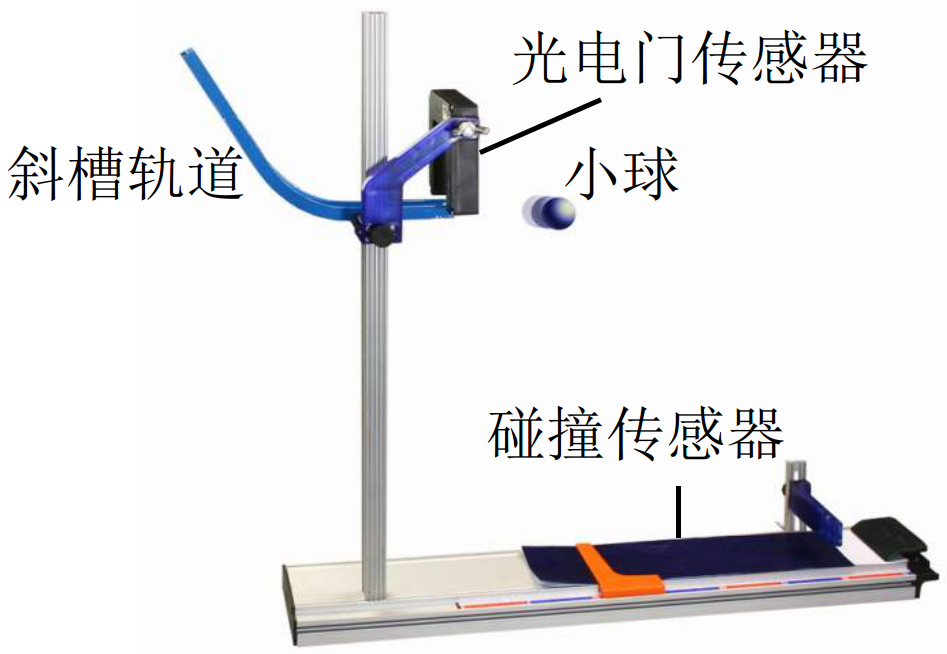
\includegraphics[width=0.3\linewidth]{picture/screenshot031}
\end{figure}

保持水平槽口距底板高度 $ h=0.420 \ m $ 不变。改变小球在斜槽
导轨上下滑的起始位置,测出小球做平抛运动的初速度 $ v_{0} $、飞
行时间 $ t $ 和水平位移 $ d $,记录在表中。
\begin{enumerate}
\renewcommand{\labelenumi}{\arabic{enumi}.}
% A(\Alph) a(\alph) I(\Roman) i(\roman) 1(\arabic)
%设定全局标号series=example	%引用全局变量resume=example
%[topsep=-0.3em,parsep=-0.3em,itemsep=-0.3em,partopsep=-0.3em]
%可使用leftmargin调整列表环境左边的空白长度 [leftmargin=0em]
\item
由表中数据可知,在 $ h $ 一定时,小球水平位移 $ d $ 与其初速度
$ v_{0} $ 成 \tk{正比} 关系,与 \tk{时间} 无关。
\begin{table}[h!]
\centering 
\begin{tabular}{|c|c|c|c|c|}
\hline 
$ v_{0} (m/s) $ & $ 0.741 $ & $ 1.034 $ & $ 1.318 $ & $ 1.584 $
\\
\hline
$ t(ms) $ & $ 292.7 $ & $ 293.0 $ & $ 292.8 $ & $ 292.9 $
\\
\hline
$ d(cm) $ & $ 21.7 $ & $ 30.3 $ & $ 38.6 $ & $ 46.4 $\\ 
\hline 
\end{tabular}
\end{table} 


\item 
一位同学计算出小球飞行时间的理论值 $t_{\text {理 }}=\sqrt{\frac{2 h}{g}}=\sqrt{\frac{2 \times 0.420}{10}}=289.8 \ ms$ 发现理论值与测量值之
差约为 $ 3 \ ms $。经检查,实验及测量无误,其原因是 \tk{$ g $ 取值 $ 10 \ m/s^{2} $ 偏大} 。

\item 
另一位同学分析并纠正了上述偏差后,另做了这个实验,竞发现测量值 $ t ^{\prime} $依然大于自己得到的理
论值 $ t ^{\prime}_{ \text{理} } $,但二者之差在 $ 3-7 \ ms $ 之间,且初速度越大差值越小。对实验装置的安装进行检查,确认斜
槽槽口与底座均水平,则导致偏差的原因是 \tk{水平槽口距底板高度 $ h $ 较大,小球飞行时受到空气阻力作用} 。


\end{enumerate}



\newpage
\item
\exwhere{$ 2014 $ 年理综安徽卷}
图 $ 1 $ 是“研究平抛物体运动”的实验装置图,通过描点画出平抛小球的运动轨迹。
\begin{figure}[h!]
\centering
\includesvg[width=0.23\linewidth]{picture/svg/GZ-3-tiyou-0448}
\end{figure}
\begin{enumerate}
\renewcommand{\labelenumi}{\arabic{enumi}.}
% A(\Alph) a(\alph) I(\Roman) i(\roman) 1(\arabic)
%设定全局标号series=example	%引用全局变量resume=example
%[topsep=-0.3em,parsep=-0.3em,itemsep=-0.3em,partopsep=-0.3em]
%可使用leftmargin调整列表环境左边的空白长度 [leftmargin=0em]
\item
以下是实验过程中的一些做法,其中合理的有
\tk{AC} 。

\fourchoices
{安装斜槽轨道,使其末端保持水平}
{每次小球释放的初始位置可以任意选择}
{每次小球应从同一高度由静止释放}
{为描出小球的运动轨迹,描绘的点可以用折线连接}

\item 
实验得到平抛小球的运动轨迹,在轨迹上取一些点,以平
图$ 1 $

抛起点 $ O $ 为坐标原点,测量它们的水平坐标 $ x $ 和竖直坐标 $ y $,图2中 $ y- x^{2} $ 图象能说明平抛小球运动轨迹为抛物线的是 \tk{C} 。
\begin{figure}[h!]
\centering
\includesvg[width=0.83\linewidth]{picture/svg/GZ-3-tiyou-0449}
\end{figure}


\item 
图 $ 3 $ 是某同学根据实验画出的平抛小球的运动轨迹,$ O $ 为平
抛的起点,在轨迹上任取三点 $ A $、$ B $、$ C $,测得 $ A $、$ B $ 两点竖直坐标
$ y_{1} $ 为 $ 5.0 \ cm $、$ y_{2} $ 为 $ 45.0 \ cm $,$ A $、$ B $ 两点水平间距$ \Delta x $ 为 $ 40.0 \ cm $。则平抛小球的初速度 $ v_{0} $ 为
\tk{$ 2.0 $} 
$ m/s $,若 $ C $ 点的竖直坐标 $ y_{3} $ 为 $ 60.0 \ cm $,
则小球在 $ C $ 点的速度 $ v_{C} $ 为
\tk{4.0} 
$ m/s $(结果保留两位有效数字,$ g $
取 $ 10 \ m/s^{2}) $。
\begin{figure}[h!]
\centering
\includesvg[width=0.23\linewidth]{picture/svg/GZ-3-tiyou-0450}
\end{figure}


\end{enumerate}






\newpage
\item
\exwhere{$ 2017 $ 年浙江选考卷}
在研究“平抛运动”实验中:
\begin{enumerate}
\renewcommand{\labelenumi}{\arabic{enumi}.}
% A(\Alph) a(\alph) I(\Roman) i(\roman) 1(\arabic)
%设定全局标号series=example	%引用全局变量resume=example
%[topsep=-0.3em,parsep=-0.3em,itemsep=-0.3em,partopsep=-0.3em]
%可使用leftmargin调整列表环境左边的空白长度 [leftmargin=0em]
\item
图 $ 1 $ 是横挡条卡住平抛小球,用铅笔标注小球最高点,确定平抛运动轨迹的方法,坐标原点
应选小球在斜槽末端时的 \tk{B} 。
\begin{figure}[h!]
\centering
\includesvg[width=0.23\linewidth]{picture/svg/GZ-3-tiyou-0451}
\end{figure}

\threechoices
{球心}
{球的上端}
{球的下端}


在此实验中,下列说法正确的是 \tk{BD} 。(多选)
\fourchoices
{斜槽轨道必须光滑}
{记录的点应适当多一些}
{用光滑曲线把所有的点连接起来}
{$ y $ 轴的方向根据重垂线确定}


\item 
图 $ 2 $ 是利用图 $ 1 $ 装置拍摄小球做平抛运动的频闪照片,由照片可以判断
实验操作错误的是 \tk{C} 。
\begin{figure}[h!]
\centering
\includesvg[width=0.16\linewidth]{picture/svg/GZ-3-tiyou-0452}
\end{figure}

\threechoices
{释放小球时初速度不为零}
{释放小球的初始位置不同}
{斜槽末端切线不水平}

\item 
图 $ 3 $ 是利用稳定的细水柱显示平抛运动轨迹的装置,其中正确的是 \tk{B} 。
\begin{figure}[h!]
\centering
\includesvg[width=0.28\linewidth]{picture/svg/GZ-3-tiyou-0453}
\end{figure}

\end{enumerate}







\end{enumerate}

